%% vedere slide Chiara di Pietro e Rosselli del turco.
\begin{frame}
	\frametitle{La comunicazione Umana}
	\framesubtitle{per comprendere la codifica bisogna partire da lontano}
	\addtocounter{nframe}{1}

	\begin{block}{In principio c'è la comunicazione}
		Comunicare è la facoltà di trasmettere qualcosa a qualcuno. Per comunicare bisogna condividere un sistema di riferimento.
		\\(Comunicare deriva dal latino communis che indica proprio la condivisione)
	\end{block}

	\begin{block}{Primo schema di base di un sistema di comunicazione}
		Qualcuno/Qualcosa che Produce; Qualcuno/Qualcosa che Trasmette; Qualcuno/Qualcosa che Consuma
	\end{block}

\end{frame}

\begin{frame}
	\frametitle{La comunicazione Umana}
	\framesubtitle{Modello della Comunicazione - C. Shannon e W. Weaver (1949)}
	\addtocounter{nframe}{1}

	\begin{center}
		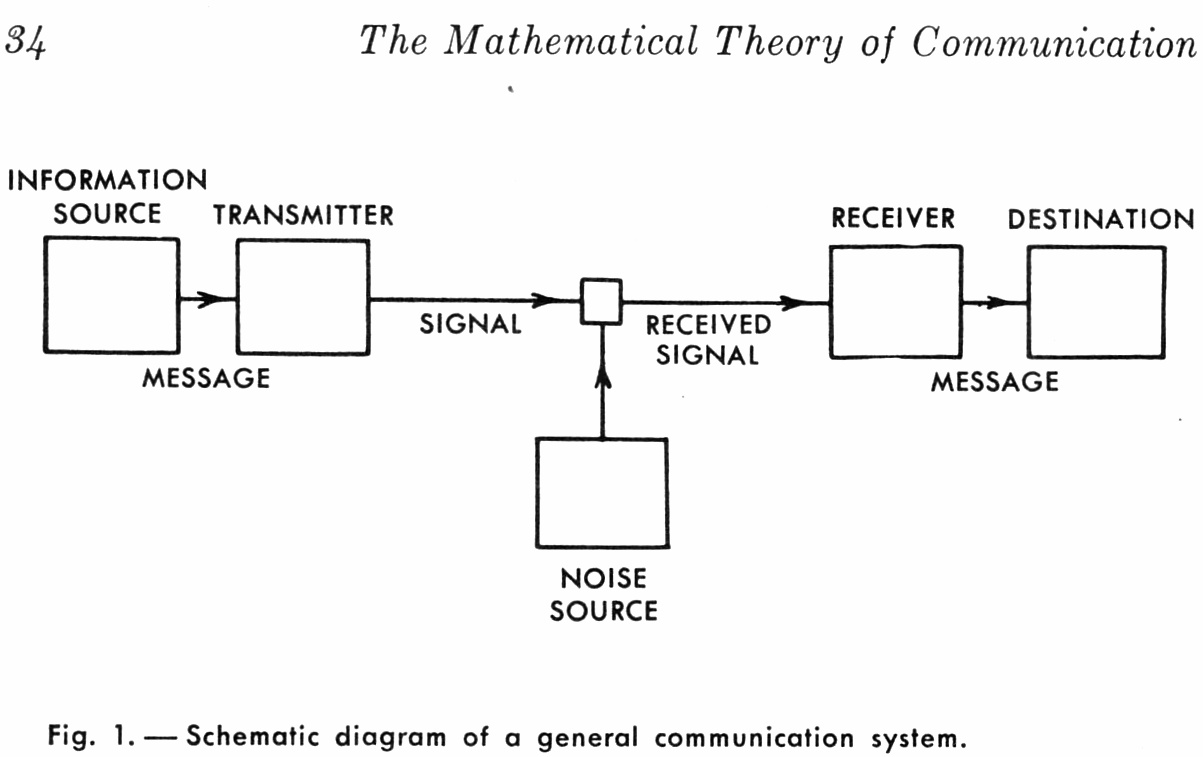
\includegraphics[width=.9\textwidth]{imgs/shannon_comm_channel.jpg}
	\end{center}

\end{frame}

\begin{frame}
	\frametitle{La comunicazione Umana}
	\framesubtitle{Modello della Comunicazione -Roman Jakobson (1966)}
	\addtocounter{nframe}{1}

	\begin{center}
		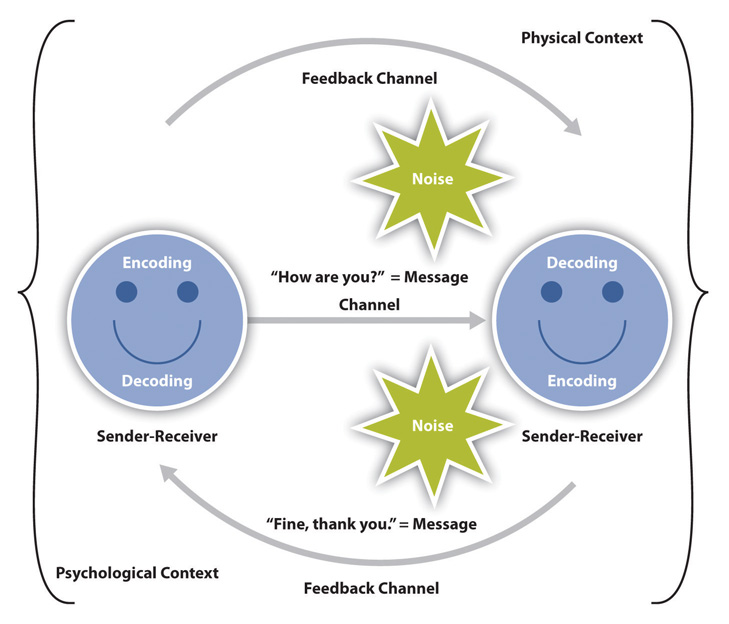
\includegraphics[width=.73\textwidth]{imgs/RomanJakobson.jpg}
	\end{center}
	\noindent\rule{5cm}{0.01cm}
	\\\tiny\url{http://open.lib.umn.edu/}

\end{frame}

\begin{frame}
	\frametitle{La comunicazione Umana}
	\framesubtitle{R. Jakobson}
	\addtocounter{nframe}{1}

	\begin{block}{Estratto Linguistics and Poetics}
		\textit{“The addresser sends a message to the addressee. To be
			operative the message requires a context referred to
			('referent' in another, somewhat ambivalent, nomenclature),
			seizable by the addressee, and either verbal or capable of
			being verbalized, a code fully, or at least partially, common to
			the addresser and addressee (or in other words, to the
			encoder and decoder of the message); and finally, a contact,
			a physical channel and psychological connection between the
			addresser and the addressee, enabling both of them to stay in
			communication.” (R. Jakobson, ‘Closing Statement:
			Linguistics and Poetics’, in Sebeok, Thomas A (Ed.) (1960):
			Style in Language. Cambridge, MA: MIT Press, p. 353)}
	\end{block}

\end{frame}

\begin{frame}
	\frametitle{La comunicazione Umana}
	\framesubtitle{R. Jackobson}
	\addtocounter{nframe}{1}

	\begin{block}{Modello Comunicazione: Funzione e Fattore}
		%\textbf{Funzione}        \textbf{Fattore}
		%\\Referenziale    Contesto
		%\\Espressiva      Mittente
		%\\Conativa        Destinatario
		%\\Fàtica          Contatto
		%\\Metalinguistica Codice
		%\\Poetica         Messaggio

		\begin{table}[]
			\begin{tabular}{lllll}
			\textbf{Funzione} & \textbf{Fattore} &  &  &  \\
			Referenziale      & Contesto         &  &  &  \\
			Espressiva        & Emittente        &  &  &  \\
			Conativa          & Destinatario     &  &  &  \\
			Fàtica            & Contatto 		 &  &  &  \\
			Metalinguistica   & Codice			 &  &  &  \\
			Poetica 		  & Messaggio        &  &  &  \\
			\end{tabular}
			\end{table}
	\end{block}

\end{frame}

\begin{frame}
	\frametitle{La comunicazione Umana}
	\framesubtitle{Diasistema}
	\addtocounter{nframe}{1}

	\begin{block}{Messaggio}
		Nel sistema della comunicazione umana non c'è una assoluta corrispondenza tra il sistema di codifica e il sistema di decodifica.
		\begin{center}
			\textit{Codice dell'agente emittente è diverso dal codice dell'agente destinatario}
		\end{center}
	\end{block}

	\begin{block}{Messaggio}
		\begin{center}
			M\textsubscript{e} != M\textsubscript{d}
			\textbf{Il Messaggio codificato è diverso dal messaggio decodificato}
		\end{center}
	\end{block}

\end{frame}

\begin{frame}
	\frametitle{La comunicazione Umana}
	\framesubtitle{Diasistema}
	\addtocounter{nframe}{1}

	\begin{block}{Diasistema - Weinreich, Uriel. - Linguista (Vilna, Polonia, 1926 - New York 1967)}
		Sistema (linguistico) di livello superiore, che riunisce due o più sistemi omogenei tra i quali ci siano somiglianze parziali (sul piano fonematico, morfologico, lessicale).
	\end{block}

	\begin{block}{Messaggio}
		Il sistema di codifica e il sistema di decodifica sono due sottosistemi di uno stesso diasistema.
	\end{block}

\end{frame}

\begin{frame}
	\frametitle{La comunicazione Umana}
	\framesubtitle{Diasistema}
	\addtocounter{nframe}{1}

	\begin{block}{Comunicazione come diasistema}
		\begin{center}Comunicazione = Sistema dell'emittente (S1) $\sim$  Sistema del destinatario (S2).\end{center}
		\textit{Il risultato di un compromesso tra il sistema S1 e il sistema S2}*
	\end{block}

	\rule{7cm}{0.015cm}
	\\*\tiny\textit{Segre, 1985}
\end{frame}

\begin{frame}
	\frametitle{Codifica del testo}
	\framesubtitle{Elementi del modello della comunicazione}
	\addtocounter{nframe}{1}

	\begin{block}{Codifica e Decodifica}
		\begin{itemize}
			\item Il termine codifica (in inglese \textit{encoding}) può essere associato alla creazione di un testo
			\item Il termine decodifica (in inglese \textit{decoding}) può essere associato alla comprensione e interpretazione di un testo
			\item Il messaggio può essere visto come contenitore di significato ($\sim$ \textit{testo})
		\end{itemize}
	\end{block}

\end{frame}

\begin{frame}
	\frametitle{Codifica del testo}
	\framesubtitle{definizioni}
	\addtocounter{nframe}{1}

	\begin{block}{Codice}
		Sistema di regole e di segni per convertire informazioni da una forma (anche astratta) in un'altra forma o rappresentazione per la comunicazione tramite un canale.
	\end{block}

\end{frame}

\begin{frame}
	\frametitle{Codifica del testo}
	\framesubtitle{Quando il destinatario è un calcolatore elettronico?}
	\addtocounter{nframe}{1}

	\begin{block}{La codifica informatica}
		Il codice deve essere in comune tra l'autore e la macchina, in un formato comprensibile ad entrambi.
	\end{block}

	\begin{block}{La codifica informatica}
		\begin{itemize}
			\item Codice in formato \textit{machine readable} (MRF), cioè un codice in formato comprensibile ad un calcolatore elettronico.
			\item Codificare per il computer implica una ricodifica del testo affinché vengano esplicitate le caratteristiche e le funzioni del testo identificate.
		\end{itemize}
	\end{block}

\end{frame}

\begin{frame}
	\frametitle{Codifica del testo}
	\framesubtitle{Esplicitare in modo formale}
	\addtocounter{nframe}{1}

	\begin{block}{La codifica informatica}
		Codificare in formato digitale un testo significa esplicitare i processi inferenziali effettuati da un interprete nella comprensione del testo stesso.
	\end{block}


\end{frame}


\begin{frame}
	\frametitle{Codifica del testo}
	\framesubtitle{Sinteticamente}
	\addtocounter{nframe}{1}

	\begin{block}{La codifica digitale di un testo}
		la codifica testuale è la rappresentazione formale di un testo e delle sue caratteristiche mediante un linguaggio informatico. (Ciotti)
	\end{block}

	\begin{block}{Grammatica formale}
		Questo linguaggio consente di rappresentare esplicitamente le caratteristiche di un testo applicando etichette meta-testuali la cui funzione e applicazione è descritta da una grammatica formale (per essere ``comprese'' da una macchina/sistema software).
	\end{block}
\end{frame}

\begin{frame}
	\frametitle{Codifica del testo}
	\framesubtitle{Linguaggio formale che diventa linguaggio teorico}
	\addtocounter{nframe}{1}

	\begin{block}{La codifica del testo come modello formale}
		La codifica digitale del testo diviene a questo punto un linguaggio teorico attraverso il quale lo studioso costruisce modelli formali del testo.
	\end{block}

	\begin{block}{Linguaggi di Markup}
		Ai fini della modellizzazione di testi, tra i linguaggi formali si sono imposti quei sistemi basati sui cosiddetti linguaggi di marcatura (\textit{markup language}).
	\end{block}
\end{frame}


\begin{frame}
	\frametitle{Codifica del testo}
	\framesubtitle{Sistema linguistico formalizzato}
	\addtocounter{nframe}{1}

	\begin{block}{Secondo Lou Burnard 1995}
		La codifica informatica di un testo impone l'adozione di un sistema linguistico formalizzato che permetta a uno studioso di rendere esplicita una interpretazione di un testo e le varie operazioni che la hanno prodotta.
	\end{block}

	\begin{block}{I sistemi dichiarativi}
		\begin{center}
			\textbf{I sistemi dichiarativi forniscono un potente dispositivo metalinguistico.}
		\end{center}
	\end{block}

\end{frame}

%Fare la codifica di un testo significa
%convertirlo in un formato comprensibile per
%l’elaboratore
%usare, a tal fine, un linguaggio di codifica di tipo
%formale
%definire e seguire uno schema di codifica ben preciso
%stabilito in base alle caratteristiche del testo che si
%intende esplicitare per il computer (modello di codifica)



%Non è codifica di un testo
%fare una scansione di un documento e diffonderne le
%immagini (ad es. in formato PDF) → digitalizzazione
%usare un software OCR per ricavarne una versione in
%formato ASCII (anche se si tratta di MRF)
%creare una pagina HTML sulla base di tale testo ASCII
%creare un documento Word ...
%creare un database testuale sulla base di tale testo
%ASCII

\begin{frame}
	\frametitle{Codifica del testo}
	\framesubtitle{Finalità}
	\addtocounter{nframe}{1}

	\begin{block}{Prerequisito per una corretta rappresentazione digitale dei testi}
		Definizione e implementazione di un linguaggio formale che deve essere sia elaborabile da un computer sia sufficientemente espressivo per rappresentare la complessità del testo.
	\end{block}

	\begin{block}{Capacità rappresentazionale}
		\begin{center}
			\textbf{Il principale requisito di uno schema di codifica, pertanto, è la capacità rappresentazionale che esso offre allo studioso}
		\end{center}
	\end{block}

\end{frame}

